\chapter{METODE PENELITIAN}
\section{Tempat dan Waktu Penelitian}
Penelitian ini dilaksanakan mulai dari bulan Februari 2025 hingga Juni
2025, bertempat di Laboratorium Elektronika dan Instrumentasi,
Departemen Fisika, Fakultas Matematika dan Ilmu Pengetahuan Alam,
Universitas Hasanuddin, Makassar.

\vspace{1em}

\section{Peralatan Penelitian}
Adapun peralatan yang digunakan pada penelitian ini adalah sebagai berikut:
\begin{enumerate}
  \item Arduino Uno berfungsi sebagai mikrokontroler utama yang
    mengendalikan motor \textit{servo} pada lengan robot serta menerima sinyal
    dari sensor.
  \item Motor \textit{servo} digunakan sebagai aktuator untuk menggerakkan
    bagian-bagian lengan robot sesuai perintah dari Arduino.
  \item Lengan robot EEZYbotARM MK1 berfungsi sebagai struktur
    mekanik yang menjadi tempat pemasangan motor \textit{servo} dan berperan
    sebagai sistem pergerakan robotik.
  \item \textit{Power supply} 5V berfungsi memberikan catu daya stabil untuk
    motor \textit{servo} agar dapat beroperasi dengan baik.
  \item \textit{Sensor Passive Infrared Receiver} (PIR) HC-SR501
    digunakan untuk mendeteksi gerakan dan membantu
    menghitung jumlah kontainer cacat dan non-cacat yang lewat.
  \item Kamera digunakan untuk mengambil gambar kontainer kimia, yang
    kemudian diproses oleh model deteksi (YOLO) dan deteksi cacat
    (\textit{autoencoder}).
  \item Laptop/komputer digunakan untuk mengunggah program ke Arduino
    Uno, serta menjalankan model deteksi berbasis YOLO dan
    \textit{autoencoder} untuk analisis visual.
  \item Kabel \textit{jumper} berfungsi menghubungkan berbagai komponen
    elektronik seperti sensor dan aktuator ke papan rangkaian dan
    Arduino.
  \item Papan rangkaian berfungsi untuk menyediakan jalur koneksi
    antar komponen.
\end{enumerate}

\vspace{1em}

\section{Metode Kerja}
Dalam penelitian ini terdapat beberapa tahapan yang harus dilakukan.
Tahapan penelitian secara lengkap dapat dilihat pada
\textit{flowchart} yang tertera pada
Gambar \ref{fig:bagan-umum}. Penelitian ini dibatasi pada perancangan
dan pembuatan prototipe sistem deteksi cacat otomatis.
\begin{figure}[H]
  \centering
  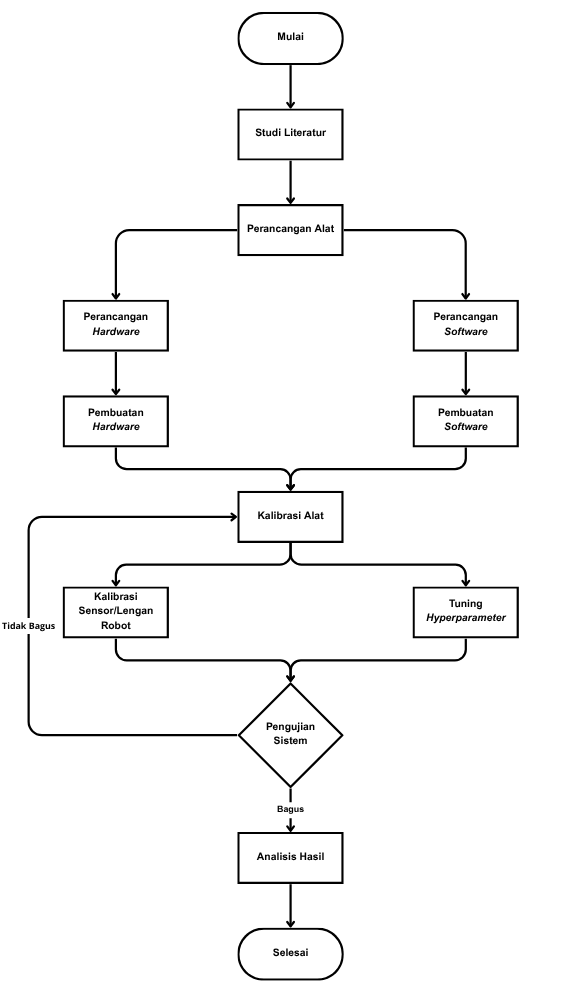
\includegraphics[width=0.7\textwidth]{gambar/bagan-umum.png}
  \caption{Bagan alir penelitian}
  \label{fig:bagan-umum}
\end{figure}
\vspace{-1em}

\begin{figure}[H]
  \centering
  \begin{tikzpicture}[
      every node/.style={font=\fontsize{9}{11}\selectfont},
      node distance = 0.67cm and 1cm
    ]
    \node (mulai) [startstop] {Mulai};
    \node (literatur) [process, below=of mulai] {Studi Literatur};
    \node (perancangan-alat) [process, below=of literatur] {Perancangan Alat};

    % Split the path relative to "Perancangan Alat"
    \node (perancangan-hardware) [process, align=center, below
    left=of perancangan-alat]
    {Perancangan \\ \textit{Hardware}};
    \node (perancangan-software) [process, align=center, below
    right=of perancangan-alat]
    {Perancangan \\ \textit{Software}};

    % Keep the parallel paths aligned
    \node (pembuatan-hardware) [process, align=center, below=of
    perancangan-hardware]
    {Pembuatan \\ \textit{Hardware}};
    \node (pembuatan-software) [process, align=center, below=of
    perancangan-software]
    {Pembuatan \\ \textit{Software}};

    %--- Here's the first trick: create a coordinate to merge the paths ---
    \coordinate (merge1) at
    ($(pembuatan-hardware.south)!0.5!(pembuatan-software.south)$);
    \node (kalibrasi-alat) [process, align=center, below=of merge1,
    yshift=-0.5cm] {Kalibrasi Alat}; % yshift to add a bit of space
    % after the merge

    % Split the path again
    \node (kalibrasi-sensor) [process, align=center, below left=of
    kalibrasi-alat]
    {Kalibrasi \\ Sensor/Lengan Robot};
    \node (kalibrasi-parameter) [process, align=center, below
    right=of kalibrasi-alat]
    {\textit{Tuning} \\ \textit{Hyperparameter}};

    %--- Second trick: use another coordinate to merge again ---
    \coordinate (merge2) at
    ($(kalibrasi-sensor.south)!0.5!(kalibrasi-parameter.south)$);
    \node (pengujian-sistem) [decision, align=center, below=of
    merge2, yshift=-0.5cm] {Pengujian Sistem};

    % Final node, perfectly centered
    \node (analisis-hasil) [process, below=of pengujian-sistem]
    {Analisis Hasil};
    \node (selesai) [startstop, below=of analisis-hasil]
    {Selesai};

    % Arrow
    \draw [arrow] (mulai) -- (literatur);
    \draw [arrow] (literatur) -- (perancangan-alat);
    \draw [arrow] (perancangan-alat) -| (perancangan-hardware);
    \draw [arrow] (perancangan-alat) -| (perancangan-software);
    \draw [arrow] (perancangan-hardware) -- (pembuatan-hardware);
    \draw [arrow] (perancangan-software) -- (pembuatan-software);
    \draw [arrow] (pembuatan-hardware) |- (kalibrasi-alat);
    \draw [arrow] (pembuatan-software) |- (kalibrasi-alat);

    \draw (kalibrasi-alat) -- (kalibrasi-alat.south |-
    kalibrasi-sensor.east);
    \draw [arrow] (kalibrasi-alat.south |- kalibrasi-sensor.east) --
    (kalibrasi-sensor);
    \draw [arrow] (kalibrasi-alat.south |- kalibrasi-parameter.west) --
    (kalibrasi-parameter);
  \end{tikzpicture}
  \caption{Bagan alir penelitian}
  \label{fig:bagan-umum-test}
\end{figure}
\vspace{-1em}

Tahapan dimulai dengan kajian mendalam terhadap teknologi robotik,
algoritma \textit{autoencoder} untuk deteksi anomali visual, serta
metode deteksi objek seperti \textit{You Only Look Once} (YOLO), guna
memperoleh pemahaman komprehensif tentang konsep dasar, format
\textit{dataset}, dan teknik perancangan model untuk mendeteksi cacat
pada kontainer kimia. Setelah pemahaman awal diperoleh, dilakukan
perancangan sistem yang mencakup perangkat keras (lengan robot dan
sensor) serta perangkat lunak berupa algoritma \textit{machine
learning}. Selanjutnya, sistem robot dikalibrasi agar dapat bekerja
secara optimal, termasuk proses \textit{tuning hyperparameter} pada
model pembelajaran mesin. Jika sistem telah berfungsi sesuai dengan
yang diharapkan, maka dilanjutkan dengan proses pengambilan data
sebagai langkah awal dalam pengujian dan validasi model.

\vspace{1em}

\subsection{Perancangan \textit{Hardware}}
Penelitian ini dimulai dengan tahap perancangan \textit{hardware}. Komponen
\textit{hardware} yang digunakan meliputi kamera untuk mengambil gambar
kontainer kimia, laptop sebagai pusat pemrosesan dan eksekusi
algoritma pembelajaran mesin, serta \textit{motion sensor} untuk menghitung
jumlah kontainer kimia, baik yang cacat maupun yang tidak. Adapun
rancangan hardware dapat dilihat pada Gambar \ref{fig:rangkaian}.

\begin{figure}[H]
  \centering
  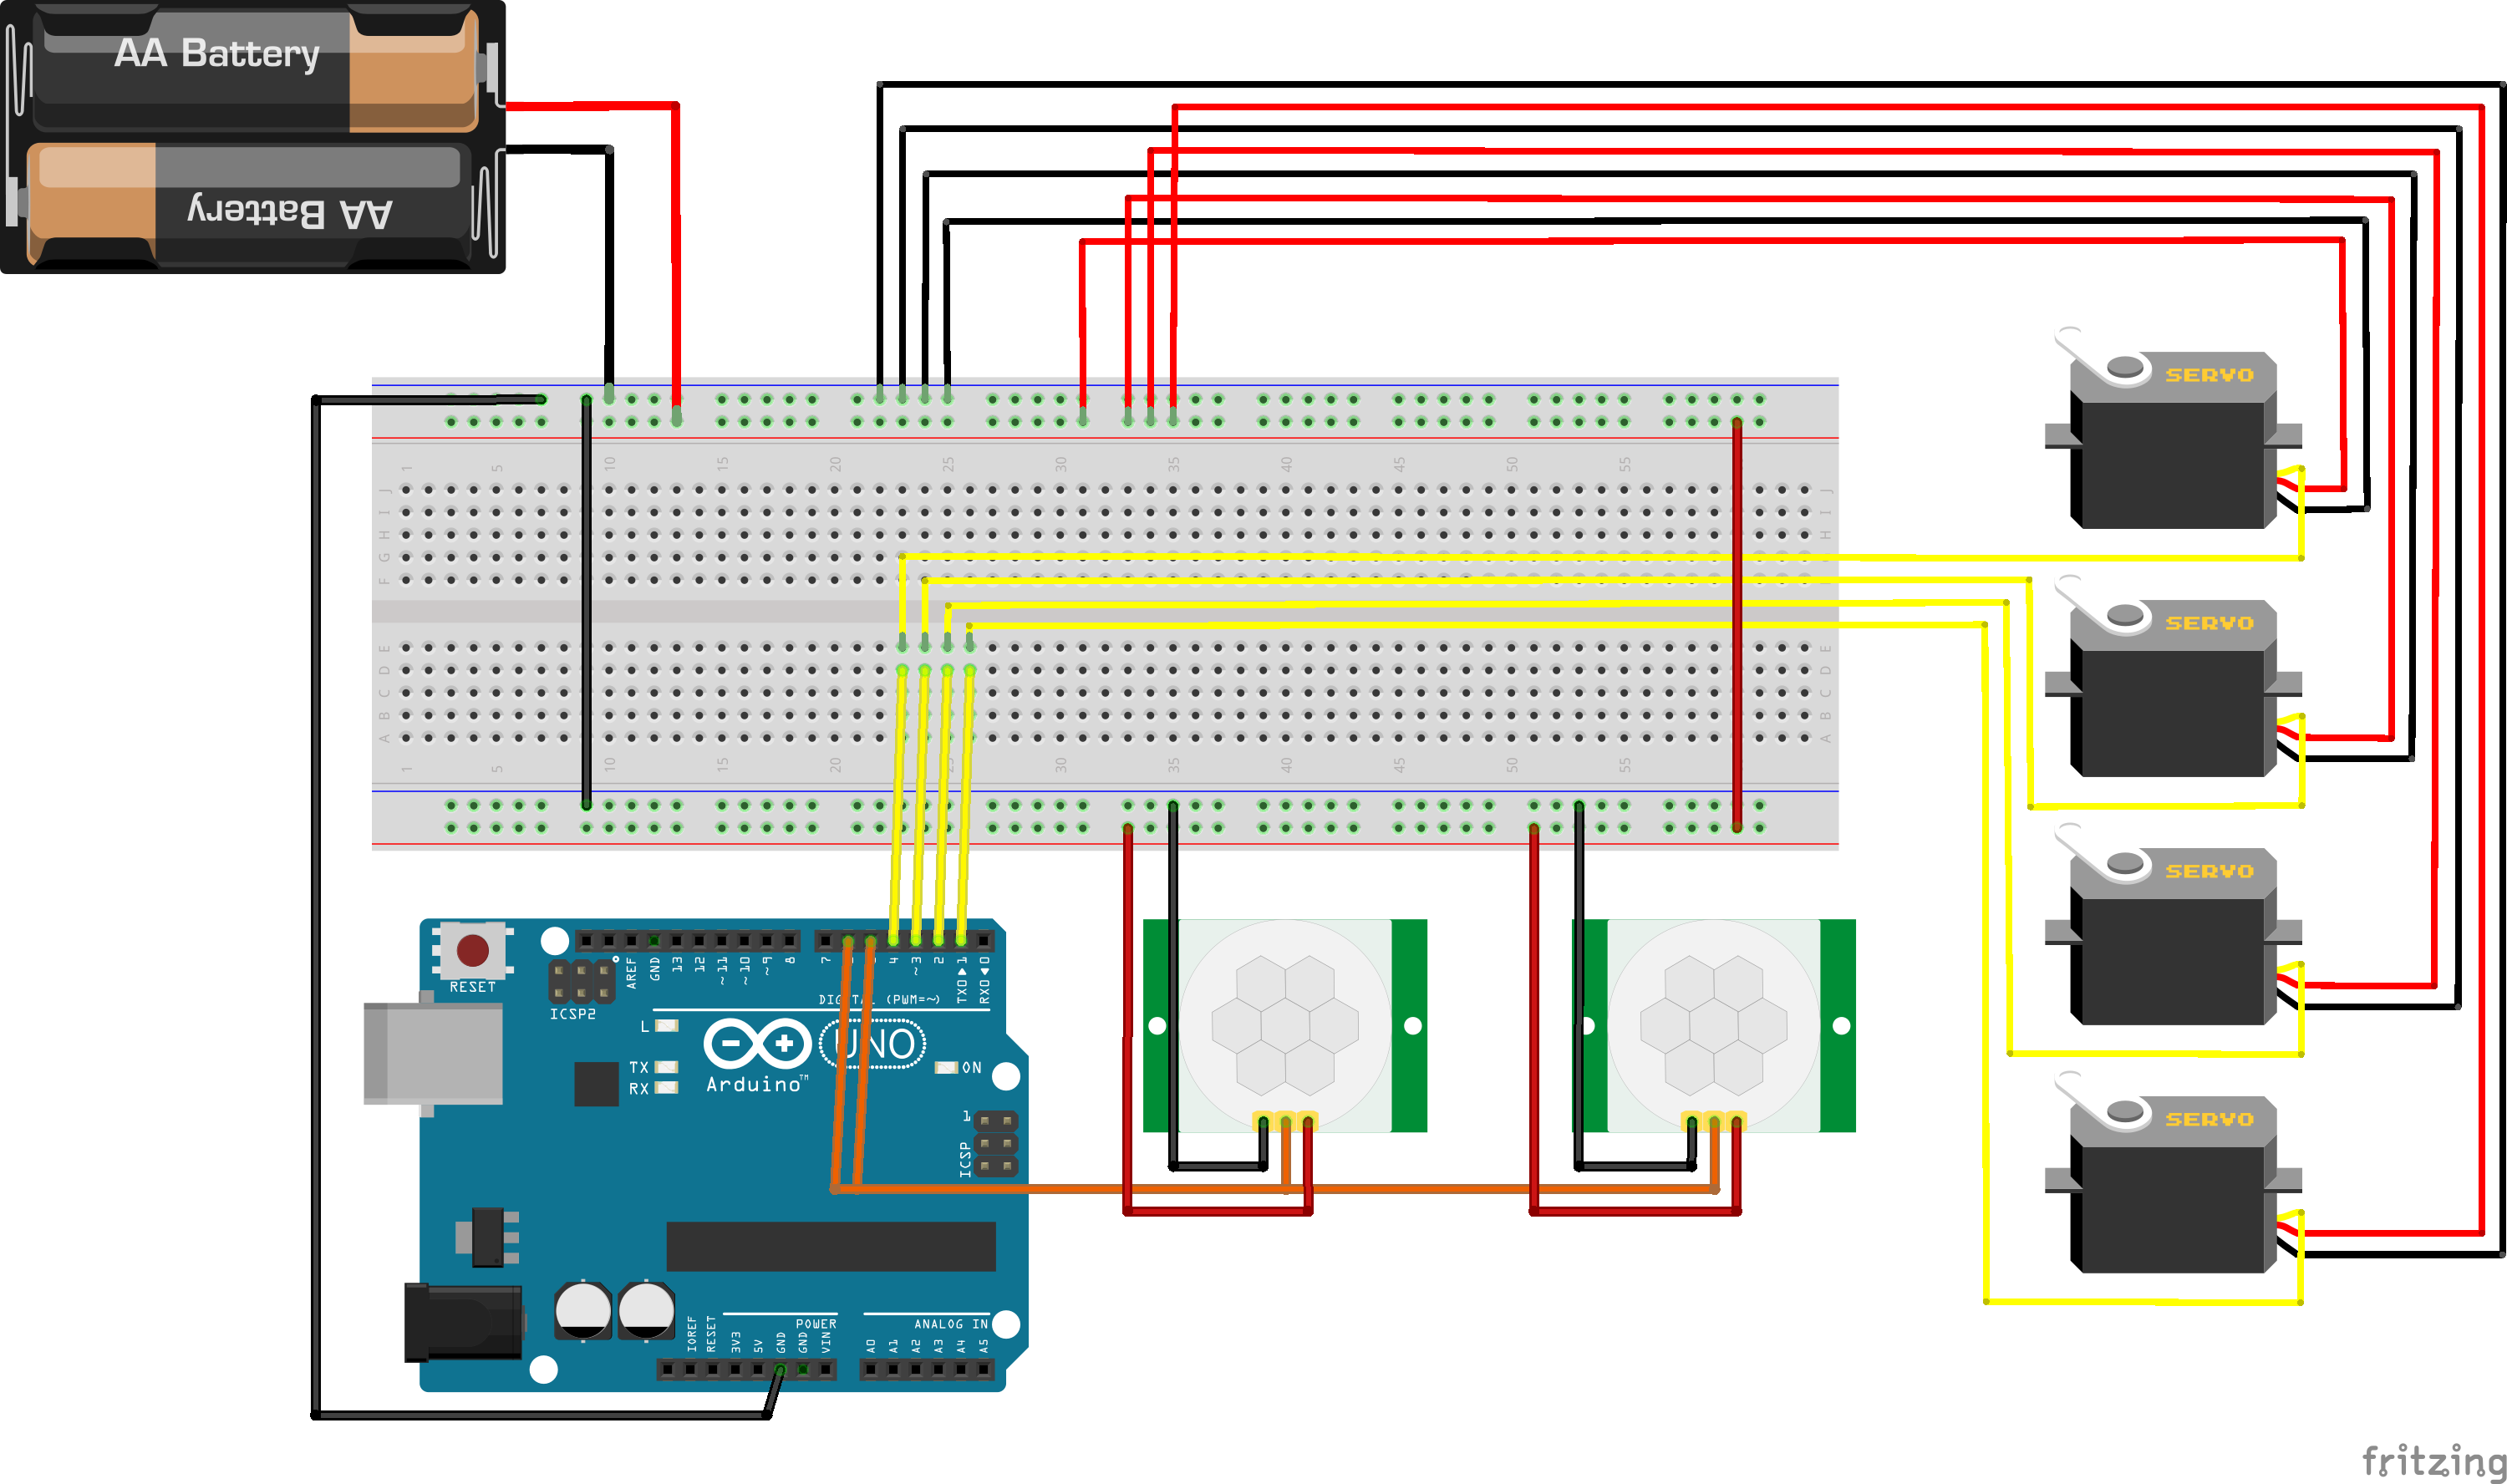
\includegraphics[width=\textwidth]{gambar/rangkaian.png}
  \caption{Bagan alir penelitian}
  \label{fig:rangkaian}
\end{figure}
\vspace{-1em}

Sistem diawali saat kamera menangkap gambar kontainer kimia yang
diletakkan di area pengambilan gambar. Gambar ini diproses oleh model
deteksi objek (YOLO) untuk mengenali keberadaan kontainer sebelum
tahap deteksi cacat. Selanjutnya, gambar yang telah dikenali dikirim
ke model deteksi kecacatan berbasis \textit{convolutional variational
autoencoder} (CVAE) untuk
menentukan apakah kontainer mengalami cacat atau tidak. Berdasarkan
hasil analisis tersebut, sinyal dikirimkan ke mikrokontroler Arduino
untuk menggerakkan \textit{servo} sebagai respon terhadap kondisi kontainer.
Lengan robot kemudian mengambil kontainer kimia dan memindahkannya ke
wadah yang sesuai, tergantung pada hasil deteksi—apakah kontainer
tersebut cacat atau tidak. Untuk memantau dan menghitung jumlah
kontainer yang telah dipindahkan, dua \textit{motion sensor} dipasang pada
masing-masing wadah (cacat dan noncacat). Data dari sensor ini
dikirim ke \textit{web server}, yang menyediakan API untuk dikonsumsi agar
data jumlah kontainer dapat ditampilkan ke klien secara \textit{real-time}.
Secara keseluruhan, keterkaitan antar komponen perangkat keras dalam
sistem ini dapat dilihat pada Gambar \ref{fig:hardware}.

\begin{figure}[H]
  \centering
  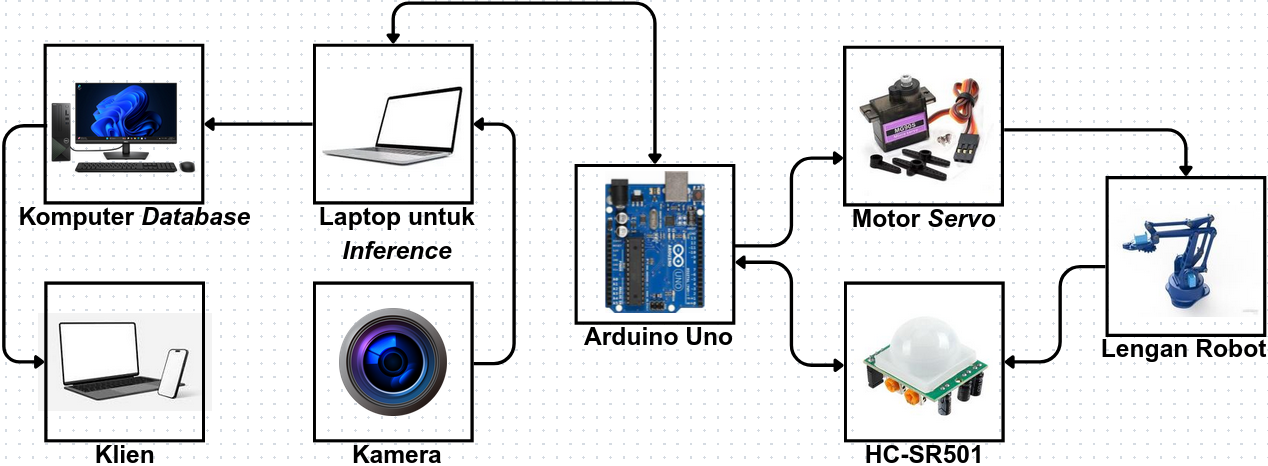
\includegraphics[width=\textwidth]{gambar/rancang.png}
  \caption{Rancang sistem \textit{hardware}}
  \label{fig:hardware}
\end{figure}
\vspace{-1em}

\vspace{1em}

\subsection{Perancangan \textit{Software}}
Perangkat lunak dalam penelitian ini mencakup perancangan beberapa
algoritma inti. Pertama, dirancang model deteksi objek berbasis YOLO
untuk mengenali kontainer kimia pada citra yang diambil oleh kamera.
Kedua, digunakan CVAE sebagai model untuk
mendeteksi cacat atau anomali visual pada kontainer. Selain itu,
dirancang pula algoritma kontrol untuk mengatur pergerakan lengan
robot dalam mengambil dan memindahkan kontainer berdasarkan hasil
klasifikasi. Sistem ini juga terintegrasi dengan modul IoT untuk
menampilkan data kontainer cacat dan non-cacat pada klien secara
\textit{real-time} melalui \textit{website}. \par

Tahap perancangan model deteksi objek dimulai dengan pengumpulan
\textit{dataset} berupa gambar kontainer kimia dari berbagai kondisi dan sudut
pandang menggunakan kamera, yang nantinya dipasang bersama lengan
robot. Setelah gambar terkumpul, dilakukan proses anotasi dengan
memberikan label dan \textit{bounding box} pada setiap kontainer sesuai dengan
format yang dibutuhkan oleh algoritma YOLO. \textit{Dataset} yang telah
dianotasi kemudian digunakan untuk melatih model deteksi objek.
Tujuannya agar model mampu mendeteksi kontainer kimia secara akurat
dan cepat dalam berbagai situasi, misalnya ketika kontainer berada
dalam posisi miring. Setelah proses pelatihan selesai, model
dievaluasi menggunakan data uji yang belum pernah dilihat sebelumnya.
Evaluasi dilakukan menggunakan beberapa metrik seperti \textit{precision},
\textit{recall}, dan \textit{mean Average Precision} (mAP), guna
memastikan bahwa model
memiliki kemampuan generalisasi yang baik dan layak diterapkan di
sistem robotik secara \textit{real-time}. \textit{Pipeline}
perancangan model deteksi
objek dapat dilihat pada Gambar \ref{fig:pipeline-yolo}.

\begin{figure}[H]
  \centering
  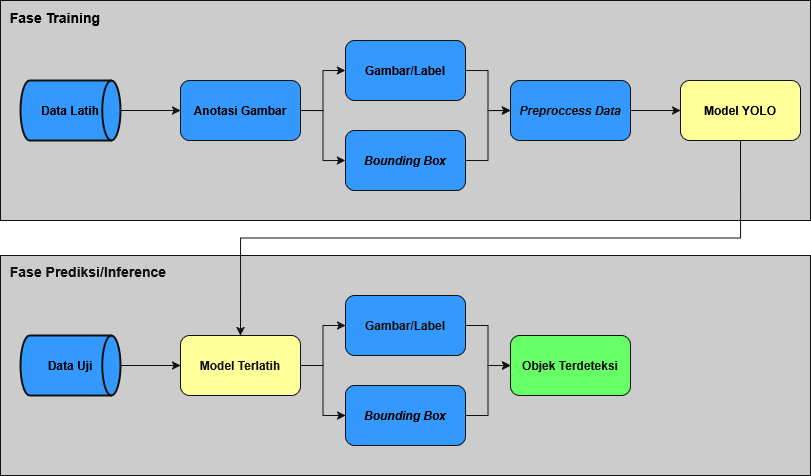
\includegraphics[width=\textwidth]{gambar/pipeline_yolo.png}
  \caption{Diagram \textit{pipeline} pelatihan model YOLO}
  \label{fig:pipeline-yolo}
\end{figure}
\vspace{-1em}

Berikutnya adalah tahap pembangunan model deteksi cacat menggunakan
algoritma CVAE. Tahap ini menggunakan
\textit{dataset}
yang sama seperti yang digunakan pada pelatihan model YOLO dengan
beberapa tambahan, namun
tanpa menggunakan anotasi \textit{bounding box} karena sifat
\textit{unsupervised} dari
\textit{autoencoder}. Data diproses melalui tahap \textit{preprocessing} seperti
\textit{resizing}, normalisasi, dan augmentasi (rotasi,
\textit{flipping}, pencahayaan)
untuk meningkatkan variasi. Model dirancang dengan dua komponen
utama: \textit{encoder} untuk mengekstraksi fitur penting dan menghasilkan
representasi berdimensi rendah (\textit{latent space}), serta
\textit{decoder} untuk
merekonstruksi gambar dari representasi tersebut. Setelah arsitektur
selesai dan data siap, model dilatih untuk meminimalkan perbedaan
antara gambar asli dan hasil rekonstruksi, sehingga mampu mengenali
citra normal secara akurat. Evaluasi dilakukan dengan menghitung
\textit{reconstruction error}, yang digunakan untuk membedakan antara gambar
normal dan cacat. Ambang batas deteksi ditentukan melalui analisis
distribusi \textit{error} pada data validasi. \textit{Pipeline}
perancangan model
deteksi cacat dapat dilihat pada Gambar \ref{fig:pipeline-autoencoder}.

\begin{figure}[H]
  \centering
  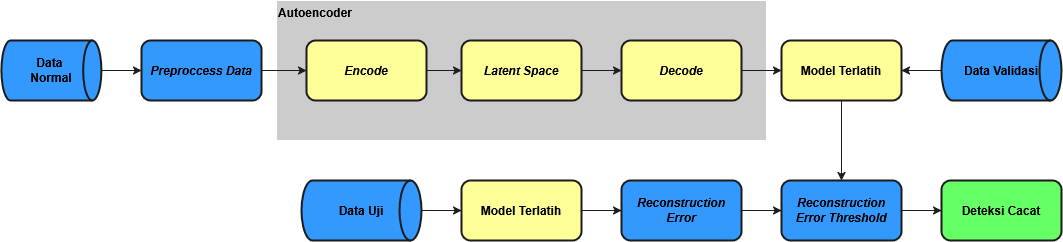
\includegraphics[width=\textwidth]{gambar/pipeline_autoencoder.png}
  \caption{Diagram \textit{pipeline} pelatihan model deteksi cacat}
  \label{fig:pipeline-autoencoder}
\end{figure}
\vspace{-1em}

\vspace{1em}

\subsection{Bagan Alir Sistem Kerja Alat}
Bagan alir kerja sistem secara keseluruhan dimulai saat kamera
menangkap citra, yang
kemudian diproses oleh model YOLO untuk mendeteksi objek kontainer.
Setelah terdeteksi, model \textit{autoencoder} menganalisis citra tersebut
untuk menentukan apakah terdapat kecacatan. Berdasarkan hasil
klasifikasi ini, lengan robot akan secara otomatis menyortir
kontainer ke lokasi yang telah ditentukan, yaitu ke area cacat jika
teridentifikasi cacat atau ke area normal jika sebaliknya.
Terakhir, informasi mengenai hasil penyortiran dikirimkan ke \textit{web
server} untuk keperluan pemantauan. Perancangan bagan alir sistem kerja
alat secara keseluruhan ditunjukkan pada Gambar \ref{fig:bagan-alir-kerja}.

\begin{figure}[H]
  \centering
  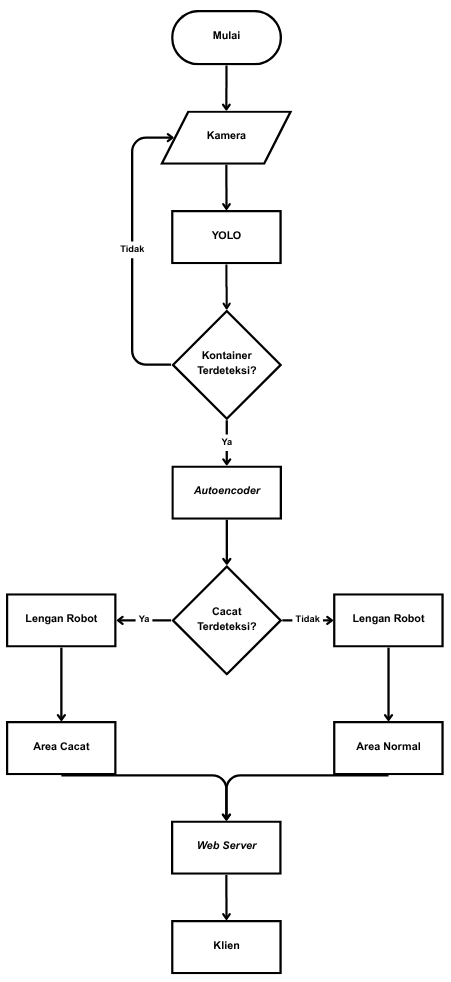
\includegraphics[width=0.7\textwidth]{gambar/flowchart.png}
  \caption{Bagan alir sistem kerja alat}
  \label{fig:bagan-alir-kerja}
\end{figure}
\vspace{-1em}
